% Discussion - Discuss the issues that you have got in the system, an idea about how you are trying to solve those. 
% Chapter Template

\chapter{Experiments, Results and Observations} % Main chapter title

\label{Chapter 5} % Change X to a consecutive number; for referencing this chapter elsewhere, use \ref{ChapterX}

\lhead{Chapter 5. \emph{Experiments, Results and Analysis}} % Change X to a consecutive number; this is for the header on each page - perhaps a shortened title

We have used Amazon AWS as serverless platform for our analysis as it is the most popular public serverless platform in use today (Source : Google Trends).

Also, our experiments mainly focus on web-based applications that use a database in the backend for which we have used AWS DynamoDB.

In addition to that, we have used AWS API gateway to generate URLs for testing purposes for exposing the lambda functions to the public.

We perform following experiments in the project :

\begin{enumerate}
    \item Traditional (IaaS) vs Serverless (FaaS)
    \item Serverless : clients spread across the globe
    \item Using cache between lambda and database
    \item Nested lambda latency
    \item Cascading lambda with different levels
\end{enumerate}

\section{IaaS vs FaaS}

In this experiment, we study latency differences of deploying a web application on dedicated servers and that with lambda functions.

\subsection{Experimental Setup}
\begin{itemize}
    \item IaaS : EC2 instances with MongoDB on backend
    \item FaaS : AWS lambda with AWS DynamoDB on backend
    \item Both lambda and DynamoDB placed at same location
    \item Locations studied : Mumbai, London, California, Canada Central, Singapore
\end{itemize}

Hypothesis : It should be same as DB and lambda deployed in the same location as EC2.

\subsection{Results}

\begin{figure}[ht]
\centering
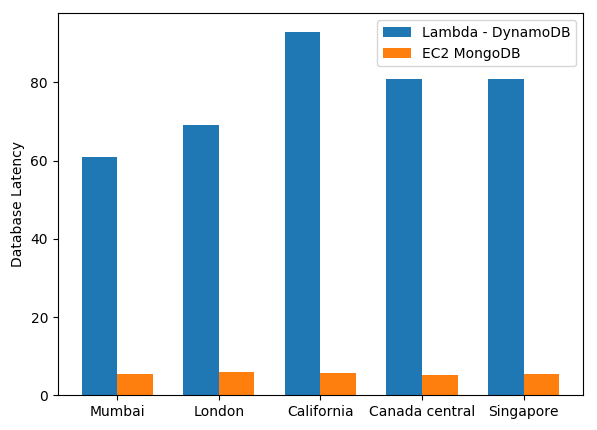
\includegraphics[height=10cm]{Images/1.png}
\caption{Huge difference between lambda and mongoDB}
\end{figure}

\subsection{Analysis}

\begin{itemize}
    \item The latency seen in FaaS is much greater than that in IaaS (approximately 6 times larger).
    \item This latency is too large (greater than 60 ms). Usually 50 ms is tolerable (Ex: in AR/VR applications)
    \item This is just a vanilla setup, the latencies are bound to increase when lambda and database are in different locations.
    \item This calls for some kind of caching mechanism which is going to be the heart of subsequent experiments.
\end{itemize}

\section{Clients spread across the globe}

In this experiment, we study latency and billing differences in invoking lambda functions when clients are present in different locations.

\subsection{Experimental Setup}
\begin{itemize}
    \item Lambda function location : Mumbai
    \item Application is simple web application using DynamoDB in the backend
    \item Clients located at India : Mumbai, USA : North California, Europe : London, Australia : Sidney, Japan : Tokyo.
    \item Used EC2 instances at different locations to emulate clients.
    \item Used AWS API gateway to expose lambda function URLs
    \item Compared 2 types of requests : POST and GET
\end{itemize}

Hypothesis : It should be different across locations due to different number of hops be across locations.

\subsection{Results}

\begin{figure}[ht]
\centering
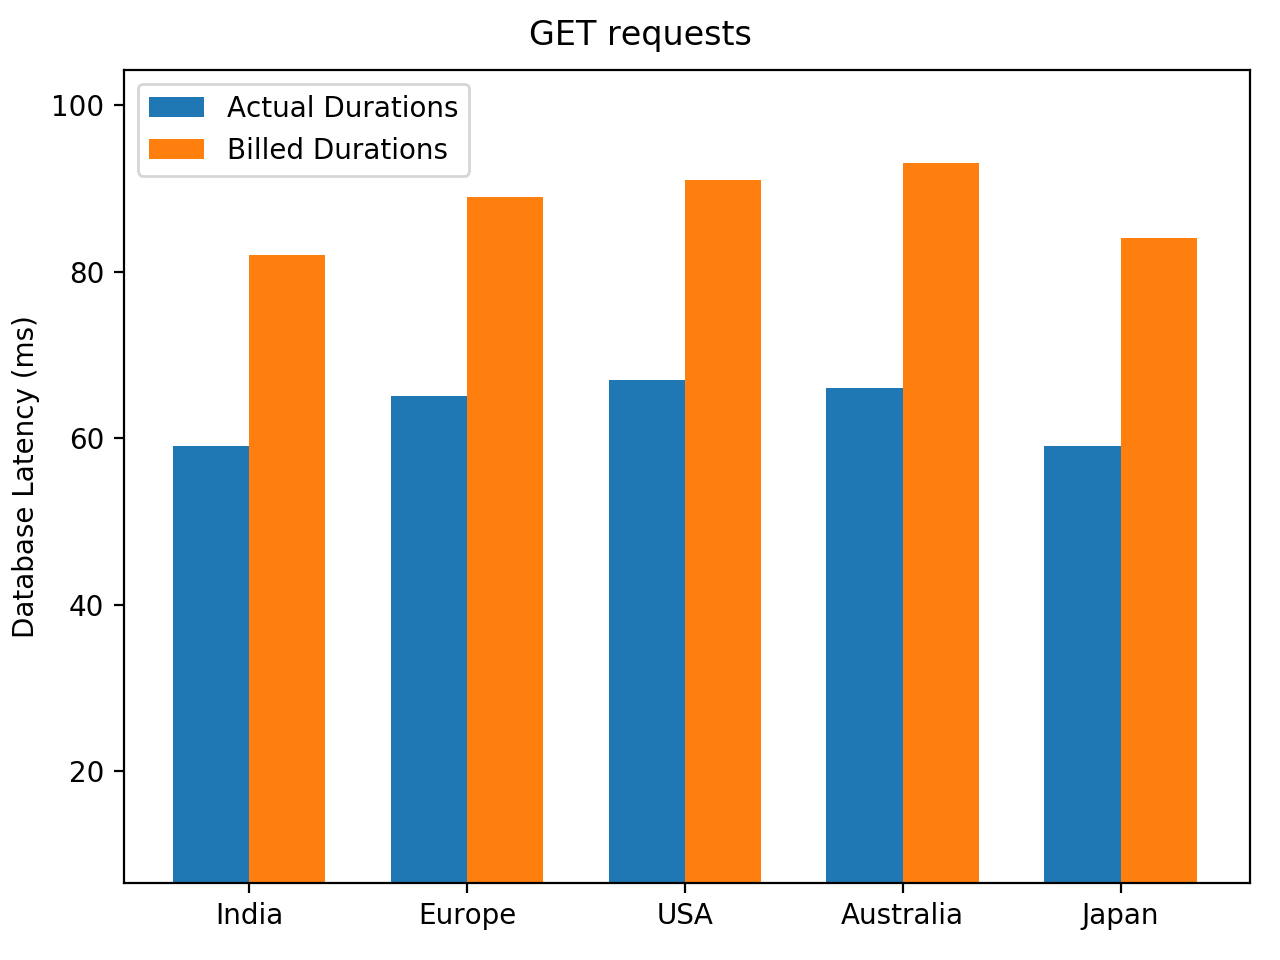
\includegraphics[height=10cm]{Images/2get.png}
\caption{Uniform difference between actual duration and billed duration}
\end{figure}

\begin{figure}[ht]
\centering
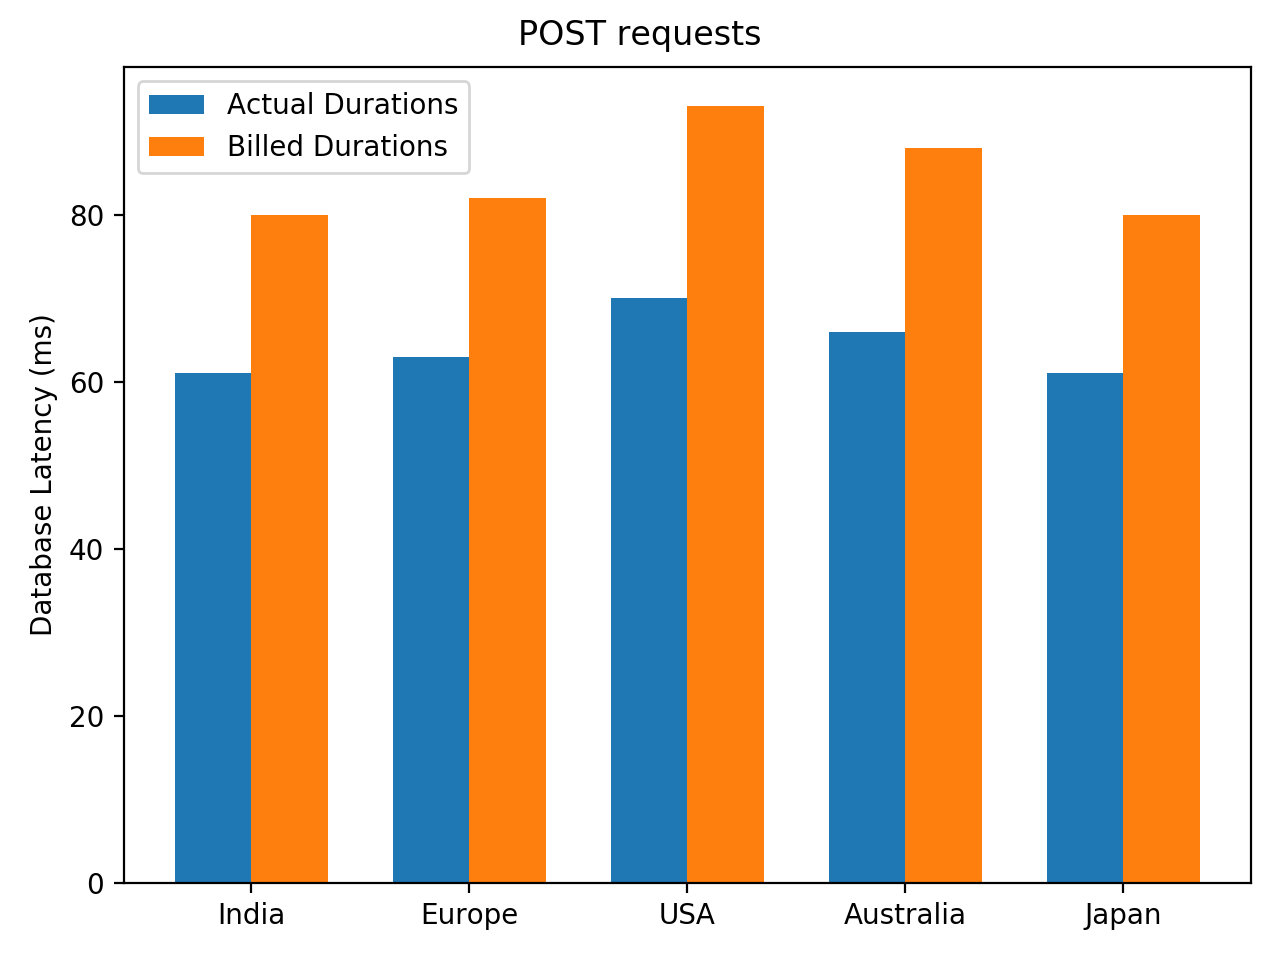
\includegraphics[height=10cm]{Images/2post.png}
\caption{Almost Similar lambda runtimes across clients}
\end{figure}

\subsection{Analysis}

\begin{itemize}
    \item The locations of client don’t affect the running time of lambda functions.
    \item The billed durations and actual duration of making a DB call is uniform across different client locations.
    \item The billed durations and actual duration do not differ much for GET and POST requests.
    \item This suggests that the client TCP connections are actually handled by API gateway exposing the lambda functions through URLs.
    \item The lambda function only receives the parameters, executes and returns the result. The client location is unknown to it.
    \item We also observe that the latency is uniformly high across different client locations.
    \item The difference between billed duration and actual DB call duration is very low compared to actual DB call duration, meaning that major portion of runtime is wasted while waiting for DB calls to return.
    \item This suggests that we can make the DB calls faster by placing some cache in between for read (GET) requests or delegating it to other lambda functions for write (POST) requests.
\end{itemize}

\section{Cache between lambda and DB}

In this experiment, we study latency differences of using various cache between lambda and DB.

\subsection{Experimental Setup}
\begin{itemize}
    \item AWS lambda
    \item For comparisons used DynamoDB directly, used Global variables as cache, used redis cache as cache
\end{itemize}

Hypothesis : Using global variables should give least latency as the variables would be stored nearest to lambda.

\subsection{Results}

\begin{figure}[ht]
\centering
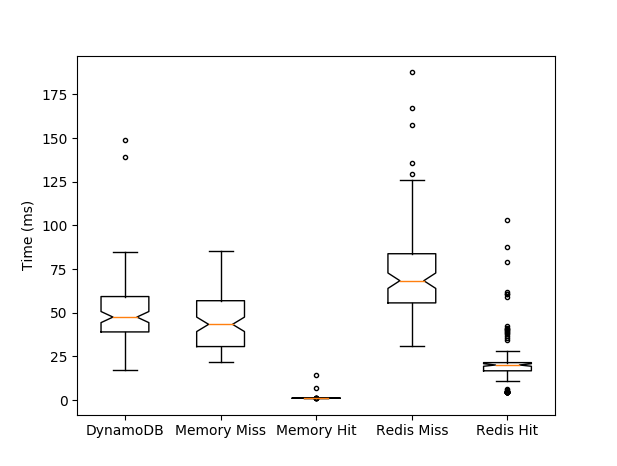
\includegraphics[height=10cm]{Images/3.png}
\caption{Global variable cache hit latency is negligible}
\end{figure}

\subsection{Analysis}

\begin{itemize}
    \item The latency seen with global variable cache is negligible.
    \item The latency in order from best to worst is global cache hit, redis cache hit, global cache miss, direct DynamoDB access and then redis cache miss.
    \item The global variables works best but it comes with a constraint. We observed that the global variables are shared only across lambda invocations within same sessions. After a cold start, the global variables are reset.
    \item Also, this problem would come when load is high and multiple containers are running at the same time. The lambda invocations in 2 different containers would be unknown to each other.
    \item Hence, it makes sense to delegate read calls for lambda too.
\end{itemize}

\section{Nested Lambda}

Here, we analyse the latency incurred when calling one lambda from another lambda.

\subsection{Experimental Setup}
\begin{itemize}
    \item AWS lambda
    \item Used a vanilla function for inner lambda
    \item Outer lambda invokes inner lambda synchronously
    \item Both lambda functions deployed at same location
\end{itemize}

Hypothesis : As the lambda functions are deployed at same location, the latency between calling one lambda from another should be negligible.

\subsection{Results}

\begin{figure}[ht]
\centering
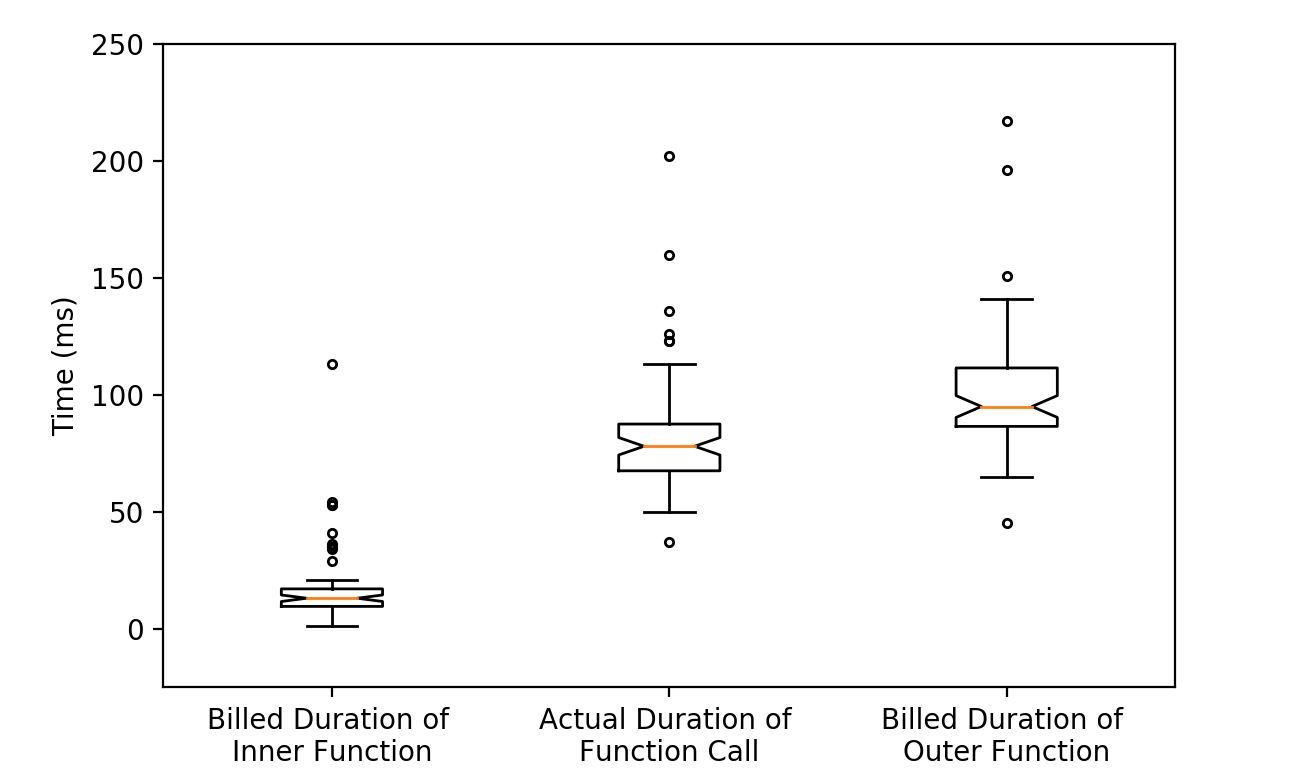
\includegraphics[height=10cm]{Images/4nested.png}
\caption{The billed duration of inner function is negligible but the actual duration of function call inside outer function is very high}
\end{figure}

\subsection{Analysis}

\begin{itemize}
    \item Billed duration of inner function is negligible as it is a vanilla function.
    \item The actual duration of function call seen inside outer function is very large. 
    \item Note that this duration will increase if there is a cache miss inside inner function during read operations.
    \item The actual duration is comparable to that of a DB call (approx 60 ms). 
    \item This suggests that some kind of queuing of requests is taking place with these invocations. 
    \item This also says that nested lambda doesn’t yield much benefit for read operations.
    \item Even though this is not beneficial for DB read operations, nested lambda is beneficial for write operations, when outer function can call inner function asynchronously and doesn’t have to wait for it to return.
    \item In the next experiment we will be seeing how latency is affected on cascading multiple lambdas at different levels.
\end{itemize}

\section{Cascaded Lambda}

Here, we analyse the latency incurred when calling nested lambda at multiple levels.

\subsection{Experimental Setup}
\begin{itemize}
    \item AWS lambda
    \item Used DB write at the innermost lambda
    \item Outer lambda invokes inner lambda synchronously
    \item All lambda functions deployed at same location
\end{itemize}

Hypothesis : As the lambda functions are deployed at same location, the latency between calling one lambda from another should be uniform.

\subsection{Results}

\begin{figure}[ht]
\centering
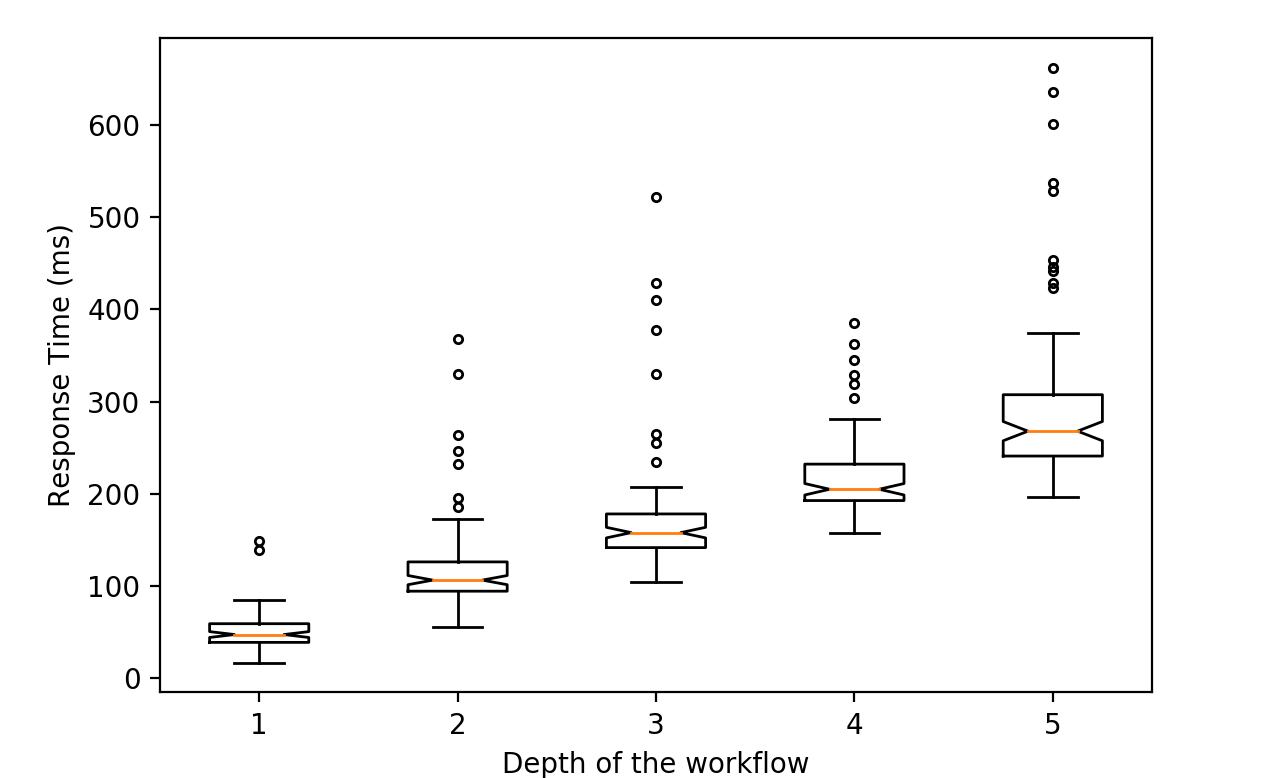
\includegraphics[height=10cm]{Images/5.png}
\caption{The latency of nested functions increases linearly with levels}
\end{figure}

\subsection{Analysis}

\begin{itemize}
    \item As we can see the nested lambda latency increases linearly across the levels.
    \item Using this information, we can increase the performance of an application using cascaded lambda by running a single lambda with all its components instead of running them one after the other.
    \item The uniform difference across different levels of lambda also strengthens the hypothesis that this latency is governed by the queuing delay at the location of deployment. 
    \item Hence, it's important to know what kind of queuing mechanism is in use.
    \item By calling same function recursively, we may be able to overcome the constraint of limited running time.
\end{itemize}